\chapter{Các thư viện lập trình OWLAPI, SWRLAPI và Vaadin framework sử dụng trong ứng dụng}
\paragraph{Giới thiệu} Chúng em xin dành chương này để giới thiệu khái quát qua các thư viện lập trình (API) và framework được sử dụng để xây dựng chương trình. Các thư viện sử dụng gồm có OWLAPI \cite{owlapi}, SWRLAPI \cite{swrlapi}, Pellet \cite{pellet}, Google Guava EventBus và thành phần giúp tạo nên giao diện người dùng của ứng dụng Vaadin Framework. Đầu tiên xin được giới thư viện lập trình OWL-API.
\section{Thư viện lập trình OWLAPI}
Thư viện lập trình Ontology Web Language là một thư viện mã nguồn mở (phát hành dưới 2 giấy phép \textbf{LGPL} và \textbf{Apache}) \cite{owlapi} được viết bằng JAVA với mục đích hỗ trợ các lập trình viên phát triển các ứng dụng có liên quan đến OWL 2 ontology. Tính đến thời điểm hiện tại thư viện đã được phát triển đến phiên bản 4.0 - cũng là phiên bản được sử dụng trong ứng dụng của chúng em.
Thư viện có các thành phần chính như sau: 
\begin{itemize}
\item API để tương tác với các thành phần của OWL 2 được đề cập trong chương 2.
\item Renderer và Parser (dùng đọc và ghi OWL 2 ontology) nhiều dạng cú pháp khác nhau đã đề cập ở chương 2 như \textit{RDF/XML}, \textit{OWL/XML}, \textit{OWL Functional Syntax}, \textit{Manchester OWL Syntax} và \textit{Turtle}.
\item Reasoner interfaces cho các reasoners khác nhau hỗ trợ cho việc suy luận.
\end{itemize}
Dưới đây là danh sách các Ontology Reasoner được hỗ trợ trong phiên bản 4.0:
\begin{itemize}
\item FaCT++ 
\item Hermit
\item Pellet \cite{pellet}
\item JFact 
\end{itemize}
Trong thư viện OWL-API, có nhiều đối tượng được xây dựng dựa trên cấu trúc phân lớp của một OWL2 Ontology, tương tự các thành phần đã được chúng em trình bày trong chương 2. Dưới đây là bảng liệt kê một số thành phần mà OWL-API đã xây dựng dựa trên mô tả trong chương 2 (chi tiết hơn ở trong \cite{owl2spec} và mã nguồn của OWL-API \cite{owlapi}).
\begin{table}
	\centering
	\begin{tabular}{|l|l|p{4cm}|}
		\hline
		Thành phần OWL 2 		& Đối tương trong OWL-API 		& Thừa kế từ đối tượng (OWL-API) \\
		\hline
		Ontology 				& OWLOntology 					& OWLObject, HasDirectImports,...  \\ 
		\hline
		Entity 					& OWLEntity 					& OWLObject,...  \\
		\hline
		Class 					& OWLClass 						& OWLClassExpression, OWLEntity, ...   \\		
		\hline
		ObjectProperty 			& OWLObjectProperty 			& OWLProperty, OWLEntity, ...   \\		
		\hline
		DataProperty 			& OWLDataProperty 				& OWLProperty, OWLEntity, ...   \\
		\hline
		NamedIndividual 		& OWLNamedIndividual			& OWLLogicalEntity, OWLEntity, ...  \\
		\hline
		Datatype 				& OWLDatatype 					& OWLDataRange, OWLPropertyRange, ...   \\
		\hline
		Property 				& OWLProperty 					& OWLLogicalEntity, OWLEntity   \\
		\hline
		ClassExpression			& OWLClassExpression			& OWLObject, OWLPropertyRange   \\
		\hline
		ObjectUnionOf			& OWLObjectUnionOf				& ClassExpression, ...\\
		\hline
		ObjectIntersectionOf	& OWLObjectIntersectionOf		& ClassExpression, ... \\
		\hline
		ObjectAllValuesFrom		& OWLObjectAllValueFrom		& ClassExpression, ... \\
		\hline
		ObjectSomeValuesFrom	& OWLObjectSomeValuesFrom		& ClassExpression, ... \\
		\hline
	\end{tabular}
	\caption{Các đối tượng OWL2 trong OWL-API\label{overflow}}
\end{table}
Trên đây chỉ là một vài thành phần, mọi thành phần OWL2 được trình bày trong chương 2 đều được OWL-API xây dựng thành các đối tượng class, interface trong JAVA để phục vụ cho việc lập trình. Tuy nhiên để tương tác với một kiến trúc đối tượng lớn và phức tạp như 1 ontology cần có cách thức chuyên dùng cho việc này là Visitor Pattern.
\subsection{Visitor Pattern}
\begin{figure}[ht!]
	\centering
	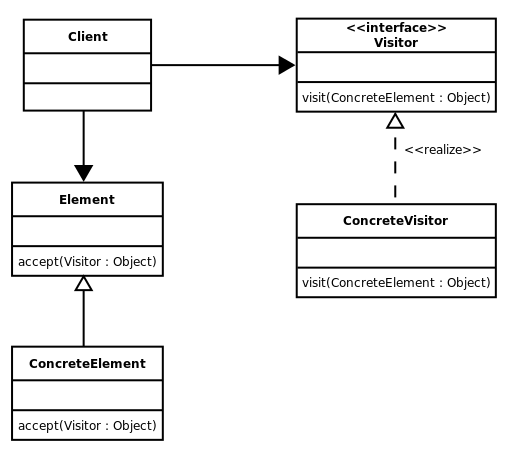
\includegraphics[width=110mm]{Figures/visitor_diagram.png}
	\caption{Visitor Diagram\label{overflow}}
\end{figure}
\paragraph{Khái quát} Trong lập trình hướng đối tượng và phát triển ứng dụng, visitor pattern hay visitor design pattern là một cách để tách biệt một giải thuật ra khỏi cấu trúc của đối tượng mà nó đang xử lý. Nhờ sự tách biệt này, chúng ta có khả năng thêm một tính năng mới cho đối tượng mà không cần phải sửa đổi cấu trúc của đối tượng đó. Lấy ví dụ là một visitor trong thư viện OWL-API là \textit{OWLClassExpressionVisitor}, chúng ta đã biết bên dưới có rất nhiều đối tượng thừa kế từ OWLClassExpression (mô tả lớp) như OWLObjectUnionOf, OWLObjectIntersectionOf, OWLClass, OWLObjectAllValueFrom, OWLObjectSomeValuesFrom, ... .Chúng ta các đoạn code như sau
\begin{verbatim}
// visitor interface
public interface OWLClassExpressionVisitor {
     public void visit(OWLClass cls);
     public void visit(OWLObjectUnionOf union);
     ...
}
// Lớp visitor
public class OWLClassExpressionVisitorImpl 
                 implements OWLClassExpressionVisitor {
    public void visit(OWLClass cls) {
        System.out.println("Lớp:" + cls.toString()); // (4)
    }
    public void visit(OWLObjectUnionOf union) {
        // Hàm getOperands trả về các mô tả lớp trong phát biểu unionOf
        for(OWLClassExpression ce: union.getOperands()) {
           ce.accept(this); // (2), (2')
        }
	}
	...
}
// Interface OWLClassExpression
public interface OWLClassExpression {
    public void accept(OWLClassExpressionVisitor visitor);
}
// Lớp OWLObjectUnionOf thừa kế từ OWLClassExpression
public class OWLObjectUnionOfImpl implements OWLClassExpression {
	public void accept(OWLClassExpressionVisitor visitor) {
    	visitor.visit(this); // (1)
    }
    ...
}
// Lớp OWLClass thừa kế từ OWLClassExpression 
public class OWLClass implements OWLClassExpression {
    public void accept(OWLClassExpressionVisitor visitor) {
        visitor.visit(this); // (3)
    }
    ...
}
// Hàm main 
public void main(String[] args) {
   OWLDataFactory factory = OWLManager.getOWLDataFactory();
   OWLClass car = factory.getOWLClass("a:Car");
   OWLClass bike = factory.getOWLClass("a:Bike");
   OWLObjectUnionOf union = factory.getOWLObjectUnionOf(car, bike);
   OWLClassExpressionVisitor visitor = new OWLClassExpressionVisitorImpl();
   union.accept(visitor);                                       
}
// Output của hàm main sẽ là 
Lớp: a:Car
Lớp: a:Bike
\end{verbatim}
Đối tượng \textit{OWLDataFactory} sẽ được trình bày ở mục sau, chúng ta có thể hiểu hàm \textit{main} như sau factory tạo ra 2 đối tượng OWLClass là car, bike tương đương với 2 lớp trong OWL2 a:Car, a:Bike, tiếp đó factory tạo ra một đối tượng union tương đương \textit{ObjectUnionOf( a:Car a:Bike )} trong OWL2. Cuối cùng ta sử dụng cho union.accept(visitor) thì thứ tự gọi hàm cho tới khi in ra từng dòng output là (1),(2),(3) và (4). 
\\
Đây chính là cách một \textit{visitor} hoạt động, thư viện OWL-API sử dụng lặp đi, lặp lại rất nhiều lần các interface visitor cho nhiều tác vụ khác nhau từ parser (dịch raw text thành cú pháp của OWL 2), renderer(dùng đọc các thành phần của ontology) như ví dụ trên qua các interface như OWLObjectVisitor, OWLDatatypeVisitor,... hoặc đọc và dịch SWRL Rule qua interface SWRLObjectVisitor. Chúng em cũng sử dụng \textit{visitor pattern} rất nhiều lần trong ứng dụng của mình để thực hiện nhiều tác vụ tương tự.
\subsection{Các hàm và đối tượng quan trọng cần biết khi sử dụng OWL-API}
\subsubsection{OWLOntologyManager}
Đây là thành phần đầu tiên cần khởi tạo trước khi chúng ta muốn nạp hay tạo một OWL2 Ontology nào, chức năng quản lý các ontology được khởi tạo, nạp. Cú pháp:
\begin{verbatim}
OWLOntologyManager modelManager = OWLManager.createOWLOntologyManager();
OWLOntolgoy ont  = modelManager.loadOntologyFromOntologyDocument(ontologyIRI);
OWLOntolgoy ont2  = modelManager.createOntology(ontologyIRI);
\end{verbatim}
\subsubsection{OWLDataFactory}
OWLDataFactory hoạt động giống như một nhà máy tạo ra tất cả đối tượng các thành phần trong OWL2 mô tả trong \cite{owl2spec} và chương 2. Cú pháp:
\begin{verbatim}
 OWLDataFactory factory = modelManager.getOWLDataFactory();
 OWLClass car = factory.getOWLClass("a:Car")
 OWLObjectProperty hasId = factory.getObjectProperty(":hasId",prefixManager);
\end{verbatim}
\subsubsection{PrefixManager}
Có chức năng quản lý các OntologyIRI, OntologyID, VersionIRI. Cú pháp
\begin{verbatim}
// Khởi tạo PrefixManger và set IRI mặc định là "DemoIRI"
PrefixManager pm = new DefaultPrefixManager(null, null, "DemoIRI#");
\end{verbatim}
\subsubsection{OWLOntology}
Là một bản mapping của OWL2 ontology thành các đối tượng trong JAVA, tất cả được lưu trong bộ nhớ (in-memory). Load ontology từ file nội bộ và URI:
\begin{verbatim}
String uri = "http://chuongdang.com/transport.owl";
File file = new File("./transport.owl");
OWLOntolgoy ont  = modelManager.loadOntologyFromOntologyDocument(IRI.create(uri));
OWLOntolgoy ont2 = modelManager.loadOntologyFromOntologyDocument(IRI.create(file));
\end{verbatim}
\subsubsection{OWLObjectRenderer}
Đảm nhiệm khả năng ghi và biên dịch các thành phần của ontology từ IRI thành dạng vắng tắt, mỗi một dạng cú pháp sẽ có một đối tượng renderer khác nhau implements OWLObjectRenderer. Ví dụ cú pháp Manchester Syntax:
\begin{verbatim}
OWLObjectRenderer renderer = new ManchesterOWLSyntaxOWLObjectRendererImpl();
// Render Class carIRI: http://Demo.org#Car
OWLClass car = factory.getOWLClass("http://vehicle.org#Car");
System.out.println(renderer.render(car));
// Output: Car
// Render ClassExpression
OWLObjectProperty buy = factory.getOWLObjectProperty("http://vehicle.org#Buy");
OWLObjectSomeValuesFrom ce = factory.getOWLObjectSomeValuesFrom(buy, car);
System.out.println(renderer.render(ce));
// Output: Buy some Car <- Manchester Syntax
\end{verbatim}
Còn rất nhiều thành phần quan trọng mà chúng em sử dụng đến trong việc phát triển ứng dụng , chúng em sẽ trình bày trong chương sau khi nói về quá trình phát triển ứng dụng phát triển ontology trên web.

\section{Vaadin Framework }
\paragraph{Giới thiệu} Vaadin Framework là nền tảng xây dựng một ứng dụng web trên Java được thiết kế giúp tạo ra một ứng dụng web chất lượng cao một cách dễ dàng nhất - tập trung chủ yếu vào one-page web application. Không giống như những framework web hiện nay đòi hỏi lập trình viên phải có kiến thức về HTML5, javascript và ít nhất một ngôn ngữ back-end. Vaadin giúp chúng ta tạm quên việc đi việc phải viết các client javascript hay từng dòng HTML để xây dựng giao diện người dùng - nói cách khác nó làm cho công việc phát triển front-end trở nên cực kì đơn giản, dễ hình dung nhất là việc phát triển một ứng dụng web trên Vaadin cũng tương tự khi chúng ta phát triển một ứng dụng desktop thông thường với các công cụ Java như AWT, Swing, hay SWT hoặc window form với C-Sharp.  Với Vaadin để phát triển được toàn bộ một ứng dụng, ngôn ngữ duy nhất chúng ta cần nắm đó là Java. Một ví dụ minh họa về tính đơn giản trong khi sử dụng Vaadin:
\begin{verbatim}
 Button button = new Button("Demo");
 button.addClickListener( new ClickListener() {
    layout.addComponent(new Label("The button was clicked"));
 }
\end{verbatim}
Đây là kết quả:
\begin{figure}[H]
 	\centering
 	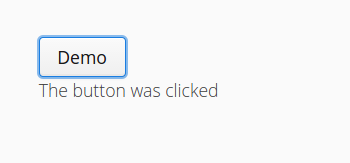
\includegraphics[width=80mm]{Figures/vaadin_democlick.png}
 	\caption{Vaadin Demo Click\label{overflow}}
\end{figure}
Thử nhìn lại nếu chúng ta xây dựng cùng chức năng trên dù là thủ công hay sử dụng các framework Web thông thường thì đều cần phải có một client script đảm nhận việc bắt sự kiện click của người dùng ở browser (front-end) và truyền nó lên server, ngay khi server nhận được (phải có đoạn code ở server "back-end" để xử lý thông tin click truyền lên từ browser), server sẽ trả về thông báo "The button was clicked", rồi front-end javascript phải thêm hay chèn một đoạn text "The button was clicked" vài HTML. Với Vaadin tác vụ vừa mô tả được thực hiện bằng đoạn code trên.
\subsection{Kiến trúc}
Vaadin hỗ trợ 2 mô hình lập trình: client và server. Mô hình lập trình phía server mạnh mẽ hơn. Mô hình lập trình phía server đảm nhận phần giao diện trên trình duyệt và giao tiếp AJAX giữa trình duyệt và server - hay nói cách khác các giao tiếp giữa server-client nhằm hỗ trợ những thao tác của người dùng đã được xử lý bởi framework và được cài đặt vào bên trong các \textit{Component} của Vaadin. Trong phạm vi ứng dụng mà chúng em xây dựng chỉ sử dụng những thành phần server - chỉ sử dụng các \textit{Component} mà Vaadin cung cấp, cộng với một vài plugin (được viết sẵn cho Vaadin) từ Vaadin Directory \cite{vaadindirectory} để giúp việc phát triển nhanh chóng hơn. 
\\
Hình sau mô tả kiến trúc cơ bản của một ứng dụng web trên Vaadin Framework. Kiến trúc ứng dụng phía server bao gồm nền tảng server (Server-side framework) và hệ thống phía client (client-side engine). 
\begin{figure}[ht!]
	\centering
	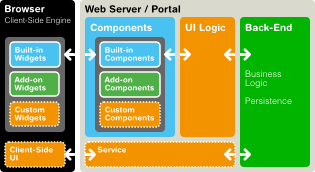
\includegraphics[width=100mm]{Figures/vaadin_architecture0.png}
	\caption{Kiến trúc của Vaadin\label{overflow}}
\end{figure}

\subsubsection{Web Server}
\begin{description}
\item[Components] Các \textit{Built-in Components}, \textit{Add-on Components} đều là những thành phần được xây dựng sẵn bởi Vaadin  hoặc được cung cấp dưới dạng các add-on từ Vaadin Directory \cite{vaadindirectory} nhằm giúp việc phát triển UI nhanh chóng hơn. Chúng đảm nhiệm back-end code để giao tiếp với các \textit{Built-in Widgets}, \textit{Add-on Widgets} ở phía browser (client side).
\item[UI Logic, Service và Custom Components] Là những phần mà lập trình viên phải tự viết code để cài đặt các tác vụ tương tác mà họ mong muốn, tuy nhiên Vaadin cũng cung cấp các abstract class, interface để hỗ trợ việc này. 
\item[Back-end] Trong một ứng dụng thông thường thì đây chính là nơi để xử lý giao tiếp với các đối tượng trong cơ sở dữ liệu - nơi thực hiện các thao tác Create
Read Update Delete (CRUD).
\end{description}
\subsubsection{Client-Side Engine}
\begin{description}
\item[Built-in Widgets] Đây chính là thành phần client-side của \textit{Built-in Components} đảm nhiệm bắt các sự kiện của người dùng với browser và giao tiếp với các \textit{Built-in Components} ở server.
\item[Add-on Widgets] là client-side của \textit{Add-on Components}.
\item[Custom-Widgets] là client-side của \textit{Custom Components}.
\end{description}
Toàn bộ các thành phần ở Client-side Engine đều được xây dựng bằng JavaScript. Đây là một ưu thế so với các nền tảng trên Flash, Java Applets hay các plugins khác. Vaadin dựa trên sự hỗ trợ của Google Web Toolkit cho nhiều trình duyệt khác nhau, nên lập trình viên không cần lo lắng về sự tương thích của các trình duyệt cho ứng dụng của mình.
\\
Như đã nói ở trên, không giống với các framework web khác là tách biệt font-end và back-end ra, Vaadin làm điều ngược lại đó là đem cả hai thứ đó tích hợp vào cái gọi là \textit{Vaadin Components}, ở hình trên chúng ta sẽ thấy một \textit{Vaadin Component} sẽ gồm một \textit{Widget} ở client-side  và một \textit{Component} tương ứng ở server side. Phân tích ví dụ Demo Click ở bên trên 
\begin{itemize}
\item \textbf{Vaadin Component} chính là một Vaadin Component.
\item \textbf{UILogic} chính là \textit{layout.addComponent(new Label("The button was clicked"));}
\end{itemize}

Tóm tắt lại, Vaadin cung cấp sẵn gần như đầy đủ mọi thành phần UI chúng ta cần để phát triển một ứng dụng web tương tác tốt với người dùng một cách nhanh chóng và tiện lợi. Chúng ta sẽ giảm bớt được công việc khi phải viết javascript, HTML cho cliend-side khi sử dụng các Vaadin UI Components.
\\
Tuy là tích hợp mọi thứ vào UI components của mình, Vaadin tách biệt UI Logic với các thiết kế giao diện. Điều này đồng nghĩa bên cạnh một giao diện mặc định rất tốt của Vaadin chúng ta có thể thiết kế giao diện một cách dễ dàng thông qua các file CSS hoặc cũng có thể tự định nghĩa HTML Template cho riêng mình \textsuperscript{*}. 
{\let\thefootnote\relax\footnotetext{*\textit{
			Vaadin Theme: https://vaadin.com/book/-/page/themes.html}}
}


%Trong hình sẽ cung cấp những thông tin chi tiết hơn về các đối tượng mà Vaadin xây dựng nhằm phục vụ cho việc thực thi các yêu cầu từ client-server và ngược lại. Mô hình trên còn được gọi là kiến trúc server-driven development.

\subsection{Vaadin UI Components}
Như đã được nhắc đến nhiều lần trong mục trước, Vaadin UI Component chính là những thành phần tạo nên Vaadin và đơn giản rất nhiều thứ khi chúng ta phát triển ứng dụng web. Dưới đây chúng em xin được nêu lên những thành phần đáng chú ý nhất. Đầu tiên xin giới thiệu thành phần quan trong nhất.

\subsubsection{User Interface} 
\paragraph{Chức năng} Ứng dụng Vaadin cung cấp một giao diện người dùng để lập trình viên có thể mở rộng ra và phát triển các chức năng mà mình mong muốn. Về mặt kĩ thuật, thành phần này sẽ được đảm nhiệm bởi các đối tượng thừa kế từ \textit{com.vaadin.ui.UI} trong source code.
\paragraph{Nhiệm vụ} Khởi tạo lớp UI, từ đây lớp UI sẽ đảm nhiệm các công việc như nạp tất cả UI Components được khai báo bên trong, cài đặt các event listener để tiếp nhận thao tác từ người dùng. Cuối cùng UI được load lên trình duyệt bằng URL, hoặc được nhúng 
vào bất kì trang HTML nào \cite{vaadinarchitecture}.
\begin{figure}[h!]
	\centering
	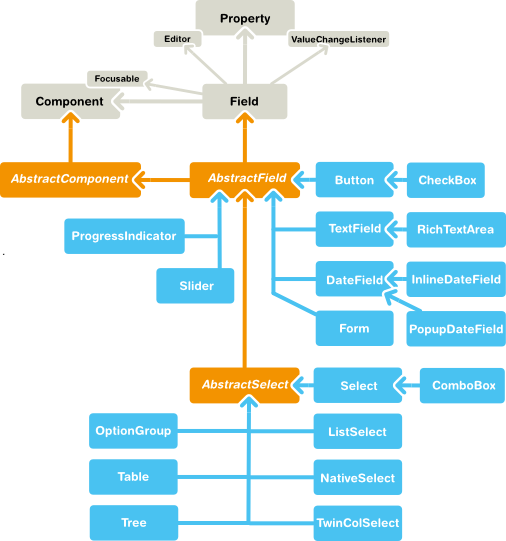
\includegraphics[width=120mm]{Figures/vaadin_architecture1.png}
	\caption{Các UI Components của Vaadin\label{overflow}}
\end{figure}

\subsection{Các thành phần đáng chú ý}
Dưới đây chúng em xin được liệt kê các Components được chúng em sử dụng nhiều trong việc phát triển ứng dụng OWLEditor.
\subsubsection{Layout}
Vaadin cung cấp nhiều dạng layout khác nhau để hỗ trợ việc tổ chức các components bên trong một cách khoa học, gọn gàng. \cite{vaadinbook}
\begin{description}
\item[HorizontalLayout] tổ chức các components theo chiều ngang, các component được sắp xếp từ trái qua phải.
\item[VerticalLayout] tổ chức các components theo chiều dọc, các component được sắp xếp từ trên xuống.
\item[AbsoluteLayout] tổ chức các components theo đúng vị trí tuyệt đối được khai báo.
\item[CssLayout] tổ chức các components theo định nghĩa từ các file css tương ứng. Đây là cách giúp chúng ta có thể tuỳ chỉnh tối đa bố cục của ứng dụng so với các layout trên.
\end{description}} 
\subsubsection{Field}
Là những components được thừa kế từ \verb|AbstractField| với chứng năng là xử lý các tác vụ input từ người dùng.
\begin{description}
\item[Button] Đảm nhiệm tính năng click từ người dùng, hành động click được xử lý bởi Button.ClickListener và ClickEvent.
\item[CheckBox] Component đảm nhiệm đánh dấu tick từ người dùng, sự kiện được xử lý bởi ValueChangeListener và ValueChangeEvent.
\item
\end{description} 


\subsubsection{Data Model}
Vaadin Data Model cho phép các view (UI components) truy xuất tới dữ liệu một cách trực tiếp, bằng cách cung cấp một interface chuẩn cho mọi loại dữ liệu. Mô hình này cho phép binding các view trực tiếp đến dữ liệu để hiển thị, và cập nhật sự thay đổi ngay lập tức khi dữ liệu được chỉnh sửa. Trong mô hình này có 3 cấp độ cấu trúc khác nhau : property, item và container.
\\
Cần lưu ý rằng Data Model không định nghĩa cách mô tả dữ liệu, mà chỉ định nghĩa interfaces cho việc binding dữ liệu đến các view. Điều này cho phép dữ liệu trong Data Model không bị giới hạn, có thể là các object Java thông thường, đường dẫn hệ thống, hoặc có thể là các câu truy vấn cơ sở dữ liệu.
\\
Data Model được sử dụng rất nhiều trong các component của Vaadin, đặc biệt là các component thừa kế interface Field hoặc AbstractField. Một tính năng đặc trưng quan trọng của các component tạo sẵn của Vaadin là nó có thể quản lý dữ liệu được gắn vào, thông qua interface Property.
\subsubsection{Properties}
Interface Property là thành phần cơ bản của Vaadin Data Model. Nó cung cấp cho đối tượng dữ liệu các phương thức đọc (get), ghi (set) cơ bản. Kiểu dữ liệu của một property có thể là bất kì lớp Java nào, và nó cũng hỗ trợ chuyển đổi giữa các kiểu dữ liệu.
\\
Phương thức setValue() dùng để ghi dữ liệu.
\\
Phương thức getValue() dùng để đọc dữ liệu.
\\
Các thay đổi của property sẽ kích hoạt sự kiện ValueChangeEvent, và được xử lý bằng ValueChangeListener. Truy xuất đến property bằng cách gọi phương thức getProperty() của event. Property thường không có định danh riêng. Chỉ khi chúng được chứa trong Item, chúng sẽ được định danh bằng các PID (Property Identifier). Tương tự, khi các Item được chứa trong Container, chúng sẽ có các định danh là các IID (Item Identifier).
\\
Mỗi component đều có một thuộc tính dùng để liên kết với nguồn dữ liệu được binding, sử dụng phương thức setPropertyDataSource() để thực hiện liên kết này.
\subsubsection{Converter}
Khi thực hiện binding, chúng ta sẽ gặp phải trường hợp kiểu dữ liệu của data khác với kiểu dữ liệu của component. Để giải quyết điều này, Vaadin cung cấp interface Converter, cho phép lập trình viên sử dụng để rạo ra các converter tuỳ theo mục đích sử dụng, để chuyển đổi kiểu dữ liệu của data sang kiểu dữ liệu hiển thị được của component. Vaadin cung cấp sẵn một vài converter thông dụng, như chuyển đổi giữa string và integer.
\subsubsection{Container}
Container là cấp cao nhất của mô hình dữ liệu Vaadin ( Vaadin Data Model ), chứa đựng và quản lý các item, trong các item lại chứa đựng và quản lý các property. Container hiển thị dữ liệu dưới dạng cấu trúc, như các dữ liệu thường thấy trong các bảng (Table), hay cây (Tree).